% ch29-fp8-persist-d.tex — FP8(二)：persist-D 主 kernel 与 scale 折叠代数（RFC-K3）★
% 源码：ffpa-attn(861d75e) cute/fp8/sm_120/persist_d.cuh(1036L) + fp8_pscale.cuh(304L)
%       + softmax.cuh(344L) + reg2reg_8b.cuh(163L) + attn_traits.cuh(313L)
\chapter{FP8（二）：persist-D 主 Kernel 与 Scale 折叠代数}\label{ch:29}

\section{本章导读}

第~\ref{ch:28}~章把 fp16 输入变成了量化 workspace（$Q_8,K_8,V_8^{\top}$ 与
scale 张量）；本章进入主 kernel——文件 \texttt{sm\_120/persist\_d.cuh} 里的
\texttt{persist\_d\_ws\_fwd\_cute\_fp8\_sm120}（sm\_120 warp-specialized
persist-D，全文件 1036 行）。它是 ffpa-attn 全仓库工程密度最高的单个文件，
也是 Part V 的\textbf{核心章}——第~\ref{ch:30}~章的 split-D / M4N2 与
第~\ref{ch:31}--\ref{ch:32}~章的 fp4 家族都建立在它引入的机制之上。

本章的主线只有一句话：\textbf{让所有量化 scale 因子要么精确消去、要么折进
本来就要做的操作}。理想境界是「除 round() 外无任何额外数学误差源」——所有
反量化都是精确代数操作，不是近似。围绕这条主线展开五组机制：
\begin{enumerate}[itemsep=0pt,topsep=2pt]
  \item \textbf{QK scale 折进 exp2 系数}：$\delta_Q\delta_K$ 与 softmax scale
        融成单个 fp32 系数，在 tile max 归约后一次乘入（29.3.1~节）；
  \item \textbf{$v_s$ 在 P 侧精确消去}：P 发射 $\tilde P = P\cdot v_s\cdot448$，
        gmem 中的 $\hat V = V/v_s$ 原样复用，$v_s$ 从 PV MMA 中代数消失
        （29.3.2~节的三步协议）；
  \item \textbf{归约轴置换不变性}：P fragment 打包零 SHFL，代价转嫁给
        $V^{\top}$ 的列置换（29.3.5~节，第~\ref{ch:28}~章预告的兑现）；
  \item \textbf{WS persist-D 结构}：128 producer + 256 consumer、
        \texttt{setmaxnreg} 32/232、Q 的 s2r 常驻与 K stage-0 复用
        （29.4.2--29.4.3~节）；
  \item \textbf{发射域纪律}：fixed $1/448$ vs per-row 满量程、lazy rescale
        与满量程互斥、f16 PV 累加域 $448\times2.25\le2047$（29.3.3--29.3.4~节）。
\end{enumerate}

\textbf{前置章节}：第~\ref{ch:17}~章（TMA+WS 双流水）、第~\ref{ch:22}~章
（TiledMMA 与 fragment）、第~\ref{ch:23}~章（swizzle）、第~\ref{ch:27}~章
（量化数学，必须）、第~\ref{ch:28}~章（前处理链，必须）。
\textbf{源码区间}：\texttt{sm\_120/persist\_d.cuh} 全文、
\texttt{fp8\_pscale.cuh} L72--300、\texttt{reg2reg\_8b.cuh} 全文、
\texttt{attn\_traits.cuh} L1--110、\texttt{softmax.cuh} L44--63；行号以
附录~\ref{app:D}~的 commit permalink 为准。
\textbf{验证方式}：\texttt{ffpa\_attn.bench} CLI，D=64/128 全绿；
D=192 本机实测发现正确性 bug（29.7.1~节的完整定位过程——这本身是本书
最有价值的一节）。预计篇幅约 18 页。

\section{问题与动机}

\subsection{主 kernel 的输入契约}

从第~\ref{ch:28}~章的 \texttt{Fp8QuantizedInputs} 出发，主 kernel 消费：
$Q_8\in$ e4m3/int8 $(N,kD)$ 行主序、$K_8$ 同构、$V_8^{\top}\in$ e4m3
$(kD,N_{pad})$ 列主序（含 \texttt{VTPerm} 置换与 16 列 TMA pad）、三组
scale（布局随粒度）、smooth-K 的 fp32 均值（lse 修正用）。主 kernel 的任务
是在 warp-specialized 流水线里完成 $O = \mathrm{softmax}(QK^{\top})V$ 的
分块在线计算，同时把 scale 的代数消去\textbf{融进流水线的每个阶段}，而不是
算完后统一反量化。

\subsection{为什么 scale 消去是核心矛盾}

低精度 MMA 只会算 $\hat P\hat V$ 这样的整数/半字节域乘累加，而 attention 的
数学在实数域。朴素的「每个操作数先乘回 scale」方案意味着每 tile 数千次
额外 FMUL 与中间张量往返——fp8 MMA 吞吐翻倍的红利会被反量化开销吃掉大半。
第~\ref{ch:27}~章 27.3.4~节给过 scale 流向总览；本章把它们逐一落到代码：
每个 scale 在哪个寄存器、哪条指令上被消去，以及哪些组合会互相冲突
（如 lazy rescale 与满量程 P）。

\subsection{persist-D 的适用域与家族分工}

persist-D 服务 $D\in\{32,64,\dots,224\}$（32 的倍数）：Q tile 整块常驻、
K/V 沿序列方向分块流过。$D$ 更大时 Q tile 无法整块驻留寄存器，交给
split-D（M8N1，$224<D<768$）与 M4N2（$D\ge768$）——见第~\ref{ch:30}~章。
本机（RTX PRO 5000）编译的 headdim 集为 $\{64,128,192,256,320,512\}$，
本章 bench 覆盖 persist-D 域内的 64/128/192。

\section{数学原理}

\subsection{QK 反量化折进 log2 域 softmax}\label{sec:29-qk-fold}

$\hat S=\hat Q\hat K^{\top}$ 是量化域（e4m3 或 int8）的整数累加，真实
$S=\hat S\cdot\delta_Q\delta_K$。softmax 需要的是
$\exp(\mathrm{scale}\cdot S)$；把 $\delta_Q\delta_K$ 与 softmax scale、
$\log_2 e$ 融成单个 fp32 系数：
\begin{equation}
  \exp\big(\mathrm{scale}\cdot\delta_Q\delta_K\cdot\hat S\big)
  =\exp_2\!\big(\underbrace{\mathrm{scale}\cdot\delta_Q\delta_K\cdot\log_2 e}_{\text{单个
  fp32 系数}}\cdot\hat S\big),
  \label{eq:29-sdequant}
\end{equation}
该系数在\textbf{tile max 归约之后}一次乘入（配合
\texttt{kMaxScaleAfter}：29.4.5~节），每元素省一次 FMUL。int8 变体走
\texttt{s8xs8$\to$s32} MMA，s32 累加器原位 cast 到 f32 寄存器后同样处理
——int8 均匀步长让小 $|S|$ 区域的相对误差更小，这是 int8 QK 在大 $N$ 下
更优的根源。

\subsection{P 量化三步协议与 $v_s$ 精确消去}\label{sec:29-pscale}

$P$ 只能在线量化（27.2.2~节「P 无法离线」）。\texttt{fp8\_pscale.cuh} 的
三步协议把 $v_s$（V 的量化 scale）从 PV 乘积中\textbf{精确}消去：
\begin{equation}
  \hat P=\mathrm{round}\!\Big(\frac{P\cdot v_s}{p_{scale}}\Big),\qquad
  \mathrm{MMA}=\hat P\,\hat V=\frac{P\,v_s}{p_{scale}}\cdot\frac{V}{v_s}
  =\frac{PV}{p_{scale}},\qquad
  O\mathrel{+}=\mathrm{MMA}\cdot p_{scale} = PV .
  \label{eq:29-threestep}
\end{equation}
$v_s$ 消去的直接推论：\textbf{gmem 中预量化的 $\hat V$ 原样复用}，主 kernel
从不需要 $V$ 的 fp16 原件；$v_s$ 被折进 P 侧的发射域
$\tilde P = P\cdot v_s\cdot448$。fixed 模式下 $p_{scale}\equiv1/448$（编译期
常数），epilogue 用 $(1/448)/\mathrm{rowsum}$ \textbf{一步}完成反量化与
归一化。

\textbf{fixed vs per-row 的取舍}：
\begin{itemize}[itemsep=1pt,topsep=2pt]
  \item \textbf{fixed（默认）}：$\tilde P = P\cdot v_s\cdot448$ 恰铺满 e4m3
        满量程；$o\_acc$ 全程单一 $448\times$ 域，rescale 可折进吸收 FFMA
        （29.4.6~节）。代价：$\max(P)\ll1$ 的平坦行（causal 顶部）只用满量程
        的一小部分。
  \item \textbf{per-row}（\texttt{FFPA\_FP8\_PQUANT\_PER\_ROW=1}）：
        $p_{scale}[row]=\mathrm{rowmax}(P)/448$ 每行满量程，精度最优；
        代价是跨 lane rowmax 归约、64-float $o\_tile$ 暂存（寄存器压力），
        且\textbf{与 lazy rescale 互斥}（29.3.3）。
\end{itemize}

\subsection{lazy rescale 的溢出约束与 fp8 的关闭}\label{sec:29-lazy}

FA-4 式 lazy rescale（27.3.6~节）允许 stale max 落后 $T$ 位才补 rescale，
期间发射的 $P$ 按 stale max 膨胀 $2^T$。fixed 模式发射域已经铺满 448，
膨胀即撞 satfinite：
\begin{equation}
  2^T\cdot\mathrm{amax}(V)\le448
  \;\Longrightarrow\;
  T=4\Rightarrow \mathrm{amax}(V)\le28 .
\end{equation}
但 ffpa 的 traits 把 fp8 的 \texttt{kLazyRescale} 直接置 \texttt{false}
（\texttt{attn\_traits.cuh} L31--37）：注释原话——跳过 rescale 会让发射 P
以最高 $2^T$ 膨胀，配合满量程发射必然 satfinite 损坏 PV。而 f16
inst\_buf 路径把 rescale 融进吸收 FFMA 后「立即 rescale 几乎免费」，
lazy 的动机（省 rescale pass）本身就消失了。\textbf{满量程与延迟 rescale
不可兼得}——这是发射域纪律的第一条。

\subsection{f16 PV 累加器的域约束}\label{sec:29-f16acc}

SA2++ 的 \texttt{mma.f16.f8.f8.f16} 让 PV 累加器走 f16 域（把 $o\_acc$
从 tensor-core 反馈链上摘下来，避开 f8f8f32 累加器 22-bit 尾数损失）。
f16 可表示范围 $\pm65504$，$m16n8k32$ 的 K 深度 32，逐元素乘积需满足
$P_r\times V_r\le65504/32=2047$。SA2++ 两侧同收（$P_r=224,V_r=4.5$）；
ffpa 的分配\textbf{只压 V 侧}：P 保持 448 满量程，per-channel V + f16 acc
时发射 $\hat V\in[-2.25,2.25]$（即 28.3.2~节的 $v_{scale\_max}=2.25$），
检验 $448\times2.25=1008\le2047$ ✓；f32 acc 时 V 侧取满 448 无约束。
kernel 侧的编译期自动收窄（\texttt{persist\_d.cuh} L723--732）：
$kBc\cdot kE4m3Max\cdot2.25\le65504$——$kBc=128$ 时 P 域被迫收到 224，
$kBc\le64$ 装得下完整 448。

\subsection{归约轴置换不变性与 reorg-free 打包}\label{sec:29-perm}

softmax 产出的 $P$ fragment（QK MMA 的 C 布局）与 PV MMA 的 A 操作数布局
\textbf{不一致}（29.4.6~节有完整布局推导）。传统解法是 16 SHFL + 32 PRMT 的
跨 lane 重排。数学出路是归约轴双射不变性：
\begin{equation}
  \sum_k P[m,k]V[k,n]=\sum_k P[m,\pi(k)]\,V[\pi(k),n]
  \qquad(\pi\ \text{任意双射}) .
  \label{eq:29-perm-inv}
\end{equation}
既然 $\pi$ 任意，就让 P \textbf{留在本 lane}、按手头字节就地打包（4 条
lane 无关 PRMT、零 SHFL），让 A 操作数携带一个置换的 k 索引 $\pi$；V 侧
在量化期按 $\pi^{-1}$ 预置换列序（\texttt{VTPermInv32}，式~\ref{eq:28-vtperm}）
——两侧槽位对上同一真实 kv 位置即可。row-sum MMA（B 为全 1）在双射下也
精确。这是「前处理链的输出布局由主 kernel 消费方式决定」的终极形态：
\textbf{一条数学等价，把 kernel 内的 16 次跨 lane shuffle 换成了量化期的
免费列置换}。

\section{设计与实现}

\subsection{traits：把配置变成类型}

\begin{lstlisting}[
  caption={persist-D fp8 traits 的关键常量（\texttt{attn\_traits.cuh} L9--42，节选）},
  label={lst:29-traits}]
// Persist-D FP8 traits: fp8 e4m3 Q/K/V via SM89 m16n8k32 mma.sync.
// V is pre-transposed by the quantize pre-kernel and stored (D x N), so the PV
// B-operand loads with the same non-transposed LDSM_N atom as Q/K; there is no
// SmemCopyAtomTransposed for fp8. TiledMma K-tile is 32 (atom K), not 16.
// kQKInt8: Q/K become symmetric int8 and QK runs SM80 m16n8k32 s8xs8->s32
// (A/B operand layouts identical to the fp8 atom; acc is s32, cast in-kernel);
// V/PV stay fp8 e4m3.
template <int kHeadDim_, typename ElementO_, int kBr_ = 128, int kBc_ = 64,
          int kStagesK_ = 2, int kStagesV_ = 2, bool kQKInt8_ = false>
struct FFPAAttnCuTePersistDFP8Traits {
  // Lazy (FA-4 deferred) rescale is OFF for fp8 precision: skipping a rescale
  // leaves the running max stale, so emitted P is inflated by up to
  // 2^FFPA_RESCALE_THRESHOLD_FP8 against that stale max; with P spanning the
  // e4m3 range (balanced narrowing) the inflation hits satfinite and corrupts
  // the PV result.
  static constexpr bool kLazyRescale = false;
  static constexpr int kSmemElems =
      kBr * kHeadDim + kStagesK * kBc * kHeadDim + kStagesV * kBc * kHeadDim;
\end{lstlisting}

四处类型决策值得注意。\textbf{其一，$V^{\top}$ 的 B 操作数用与 Q/K 相同的
非转置 LDSM\_N atom}：V 已在 gmem 里转置好，kernel 里没有转置视角。
\textbf{其二，TiledMma 的 K-tile 是 32}（atom 的 k16$\times$2），fp16 家族
是 16。\textbf{其三，swizzle atom 按行字节选}（L45--50）：Q/K 行 $D$ 字节、
$V^{\top}$ 行 $kBc$ 字节，各自落 SW128/SW64/SW32——一图两制。
\textbf{其四，kBc 随 D 切换}：launcher 对 $D\le128$ 实例化 $kBc{=}128$、
$D>128$ 用 64（smem 预算）。

\subsection{WS 骨架与 smem 复用}

128 线程 producer（TMA 装载）+ 256 线程 consumer（全部计算），
\texttt{\_\_launch\_bounds\_\_(384,1)}；寄存器经 \texttt{setmaxnreg}
重分配——producer 释放到 32，consumer 拿到 232。fp8 路径的 consumer
无条件拿 232（fp16 版在 D=128 时只需 170）：P 量化 + row-sum + rescale
状态把寄存器压力抬上来了，注释记录「静态 170 上限会 spill 约 60 个寄存器」。

\begin{lstlisting}[
  caption={Q smem 复用与槽位轮转（\texttt{persist\_d.cuh} L193--215，节选）},
  label={lst:29-smem}]
  // SMEM: [Q | K stages | V stages], 1B per elem (int8 or e4m3). With
  // kPersistQs2r the Q tile is read into regs once before the kv loop, so
  // its 16KB area (slot 0 of the K region) is reused by the LAST K stage
  // and the Q bytes drop out of the allocation: smem = (kStagesK +
  // kStagesV) K/V tiles, e.g. stages 2 -> 64KB (vs 80KB keeping a dead Q
  // tile). The saving buys L1, not occupancy: smem/L1 share one pool per SM
  // (~4-5us per 16KB), and residency stays register-limited (1 CTA/SM)
  // either way.
  // kPersistQs2r slot rotation: logical stage s -> physical slot (s+1) %
  // kStagesK, so the Q area (slot 0) hosts the LAST stage. That stage's
  // first TMA issue happens in steady state (k_tile == kStagesK-1) and its
  // first consume is tile kStagesK-1, hiding the q_consumed wait behind a
  // full tile of compute; the prologue stages (slots 1..) never touch the
  // Q area and issue with no Q dependency at all.
  constexpr auto kKSlot = [](int s) {
    return kPersistQs2r ? (s + 1) % kStagesK : s;
  };
\end{lstlisting}

两层设计叠加。\textbf{Q 的 s2r 常驻}（\texttt{kPersistQs2r} 默认 true）：
Q 在 kv 循环前一次性读进寄存器，之后 QK 步骤全是 gemm\_rs（K-only smem 读）
——D=128 实测 $-8\mu s$、零 spill；Q 的 smem 区（slot 0）随即死亡。
\textbf{槽位轮转}让复用区承接「最后一个 K stage」而非第一个：它的首次 TMA
发射与首次消费都发生在稳态（隔着一整 tile 计算），\texttt{q\_consumed} 的
等待被完全藏住。省下的 16KB smem 买的是 L1 容量而非 occupancy——smem/L1
共池，实测每 16KB $\approx$ 4--5$\mu s$，而 CTA 驻留本就被寄存器锁在
1/SM。

producer 的装载序还有两处细节：\texttt{V prologue 先于 K}（V0 只在
QK0+softmax 之后才被消费，先发永远安全）；consumer 在等 Q 之前先
\texttt{arrive} 全部初始 \texttt{k\_empty}/\texttt{v\_empty}（这些 arrive
不依赖 Q 数据，提前放行让 K(0)/V(0) 的 TMA 与 Q 的 TMA inflight中重叠）。

\subsection{主循环：五个 Phase 的字节旅程}

consumer 的 kv 循环（\texttt{\#pragma unroll 1}，逐 tile）：

\textbf{Phase 1 -- QK GEMM}（L583--601）：等 \texttt{k\_full}、fence、
\texttt{gemm\_rs(tCrS, tCrQ, tCrK, ...)}——Q 在寄存器、K 从 smem 流入。
int8 变体把 s32 累加器\textbf{原位} cast 成 f32（复用同一组 4B 寄存器），
零额外寄存器。scale 粒度在读取处分叉：per-block 的 $k_s$ 是每 tile 一个
标量；per-thread 的 $k_s$ 按
\texttt{(wg\_tid\%32)\%4} 列组查表（4 scale/块，SM80\_16x8 C-fragment 的
lane$\to$列对映射），$q_s$ 按行查 \texttt{qs\_arr[row]}
（$\{r,r{+}8\}$ 行对共享）。

\textbf{Phase 2 -- log2 域 softmax}（L649--790）：mask（causal
tail-aligned 的 \texttt{mask\_start\_tile}/\texttt{Tc\_eff} 两级剪枝，
尾 tile 内逐元素 $-\infty$）；随后
\texttt{online\_softmax\_fp8\_fixed} 以 $\log_2(p\_quant\_scale)$ 为
exp2 偏移，softmax \textbf{直接发射} $\tilde P = P\cdot v_s\cdot448$——
式~\ref{eq:29-threestep} 的 (1) 步折进 softmax 本身。\texttt{kMaxScaleAfter}
（int8+f16acc 配置）：tile max 用未 scale 的原始 scores 归约、跨 lane
归约完成后一次乘 $\delta_Q\delta_K\cdot$scale——max 临界路径上每元素省
一次 FMUL。

\textbf{Phase 3 -- P 打包}（L813--831）：

\begin{lstlisting}[
  caption={P$\to$e4m3 A 操作数的双路径（\texttt{persist\_d.cuh} L813--831）},
  label={lst:29-pack}]
    // P -> e4m3 A operand (see fp8_pscale.cuh). Per-row mode needs the row
    // max first, then scales+converts; fixed mode was pre-scaled by the
    // softmax and only converts (packed e4m3x2) + reorgs. kReorgFree swaps
    // the cross-lane reorg for the shuffle-free perm pack (paired with the
    // permuted V^T written by the quantize pre-kernel).
    if constexpr (kReorgFree) {
      PackC8bitToA8bitPermVT perm_pack;
      if constexpr (kPQuantPerRow) {
        pscale_per_row(scores, p_scale);
        quantize_p_frag<true>(scores, tCrSf, vs, p_scale, perm_pack);
      } else {
        quantize_p_frag_prescaled(tCrSf, perm_pack);
      }
    } else if constexpr (kPQuantPerRow) {
\end{lstlisting}

fixed 模式下 softmax 已经发射满量程值，pack 只做 f32$\to$e4m3x2 打包 +
寄存器重排——\texttt{kReorgFree} 选择 29.3.5~节的置换打包（4 PRMT、
零 SHFL），fallback 的跨 lane \texttt{ReorgC8bitToA8bit} 保留编译、
由 split-D 家族继续使用。

\textbf{Phase 4 -- row-sum 与 PV GEMM}（L833--903）：先在 tensor core 上
跑 \texttt{pscale\_rowsum\_mma}（B 操作数全 1 的 MMA 求行和，NCU 显示它
藏进 PV 的 tensor pipe 气泡，CUDA-core FADD/shfl 版本实测更慢）。PV 主体
分三路：f32 acc 直接 \texttt{gemm\_rs(o\_acc, tCrP, tCrV, ...)}；
\textbf{f16 acc} 路线是本章最精彩的指令级融合——PV 先累进 f16
\texttt{inst\_buf}（把 $o\_acc$ 摘出 tensor-core 反馈链），随后吸收回
f32 $o\_acc$ 时用 FFMA 把 online-softmax 的 rescale 一起折进去：
\begin{equation}
  o\_acc \leftarrow \mathrm{FFMA}(o\_acc,\ row\_scale,\ float(inst\_buf)),
\end{equation}
\texttt{row\_scale} 恰为 1.0 的行（阈值跳过）免乘——独立的 rescale pass
整个消失。

\textbf{Phase 5 -- epilogue}（L904--1031）：$O = o\_acc\cdot(1/448)/
\mathrm{rowsum}$（fixed 单步反量化+归一化）；per-channel V 按 D 列查
$v_{s,d}$ 逐列消去、smooth-V 加回 $\bar v_d$；lse $=$
$(\mathrm{rowmax}+\log_2\mathrm{rowsum})\ln2$，smooth-K 的修正
$+\mathrm{scale}\cdot q_s\cdot q_{km}$（28.4.2~节的点积在循环外预算）。
输出走 \textbf{STSM 进已释放的 smem（Q/K/V 全部消费完）再 TMA store}——
一次合并写出；尾 tile（不满 128 行）退化为带行守卫的直接 R$\to$G 写。

\subsection{reorg-free 打包的布局推导}

\begin{lstlisting}[
  caption={C$\to$A 重排为什么必要（\texttt{reg2reg\_8b.cuh} L14--34，节选）},
  label={lst:29-reorg-bg}]
// The QK C-fragment and the PV A-fragment distribute a 16x32 tile over the
// warp DIFFERENTLY (PTX ISA, "Matrix Fragments for mma.m16n8k32"; with
// groupID g = lane>>2 and threadID_in_group t = lane&3):
//   C fragment (4 regs c0..c3, one value each; 2 cols per row):
//     c0,c1: row g,   cols {2t, 2t+1}
//     c2,c3: row g+8, cols {2t, 2t+1}
//   A fragment (4 regs a0..a3, four 8-bit elems each; 4 k-cols per row):
//     a0: row g,   k = 4t..4t+3
//     a1: row g+8, k = 4t..4t+3
//     a2: row g,   k = 16+4t..16+4t+3
//     a3: row g+8, k = 16+4t..16+4t+3
//     => thread t needs k-columns {4t..4t+3} which, expressed in the C-tile
//        column pairs {2t',2t'+1}, belong to OTHER lanes (e.g. t=1 needs the
//        bytes owned by t=2 and t=3). A purely in-thread permutation cannot
//        build the natural A layout (proven in .tmp/fp8_persist_d/
//        verify_layouts.py), hence the cross-lane ReorgC8bitToA8bit below.
\end{lstlisting}

C fragment 里 lane $t$ 持列对 $\{2t,2t{+}1\}$，A fragment 却要列
$\{4t,\dots,4t{+}3\}$——后者横跨多个 lane 的字节。\texttt{ReorgC8bitToA8bit}
用 16 SHFL + 32 PRMT 跨 lane 凑齐；而 \texttt{PackC8bitToA8bitPermVT}
（L96--141）反问：为什么要凑\textbf{自然}布局？就地打包后 A 槽位
$s$ 持真实列 $\pi(s)$（$\pi = [0,1,8,9, 2,3,10,11,\dots]$，每 32 列周期），
V$^{\top}$ 列按 $\pi^{-1}$ 预置换即可。四个 \texttt{\_\_byte\_perm}
选择器（0x5410/0x7632/0xDC98/0xFEBA）\textbf{lane 无关}——没有构造器
状态、没有分支，且与 \texttt{ReorgC8bitToA8bit} 的对照已用 pycute 数值
验证布局等价。注释末尾的 CONTRACT 加了感叹号：\textit{this pack must
NEVER run against an unpermuted V\^{}T}——配对由 launcher 的单一
\texttt{reorg\_free} 编译期常量强制，两侧永不发散。

\section{图示}

\begin{figure}[H]
  \centering
  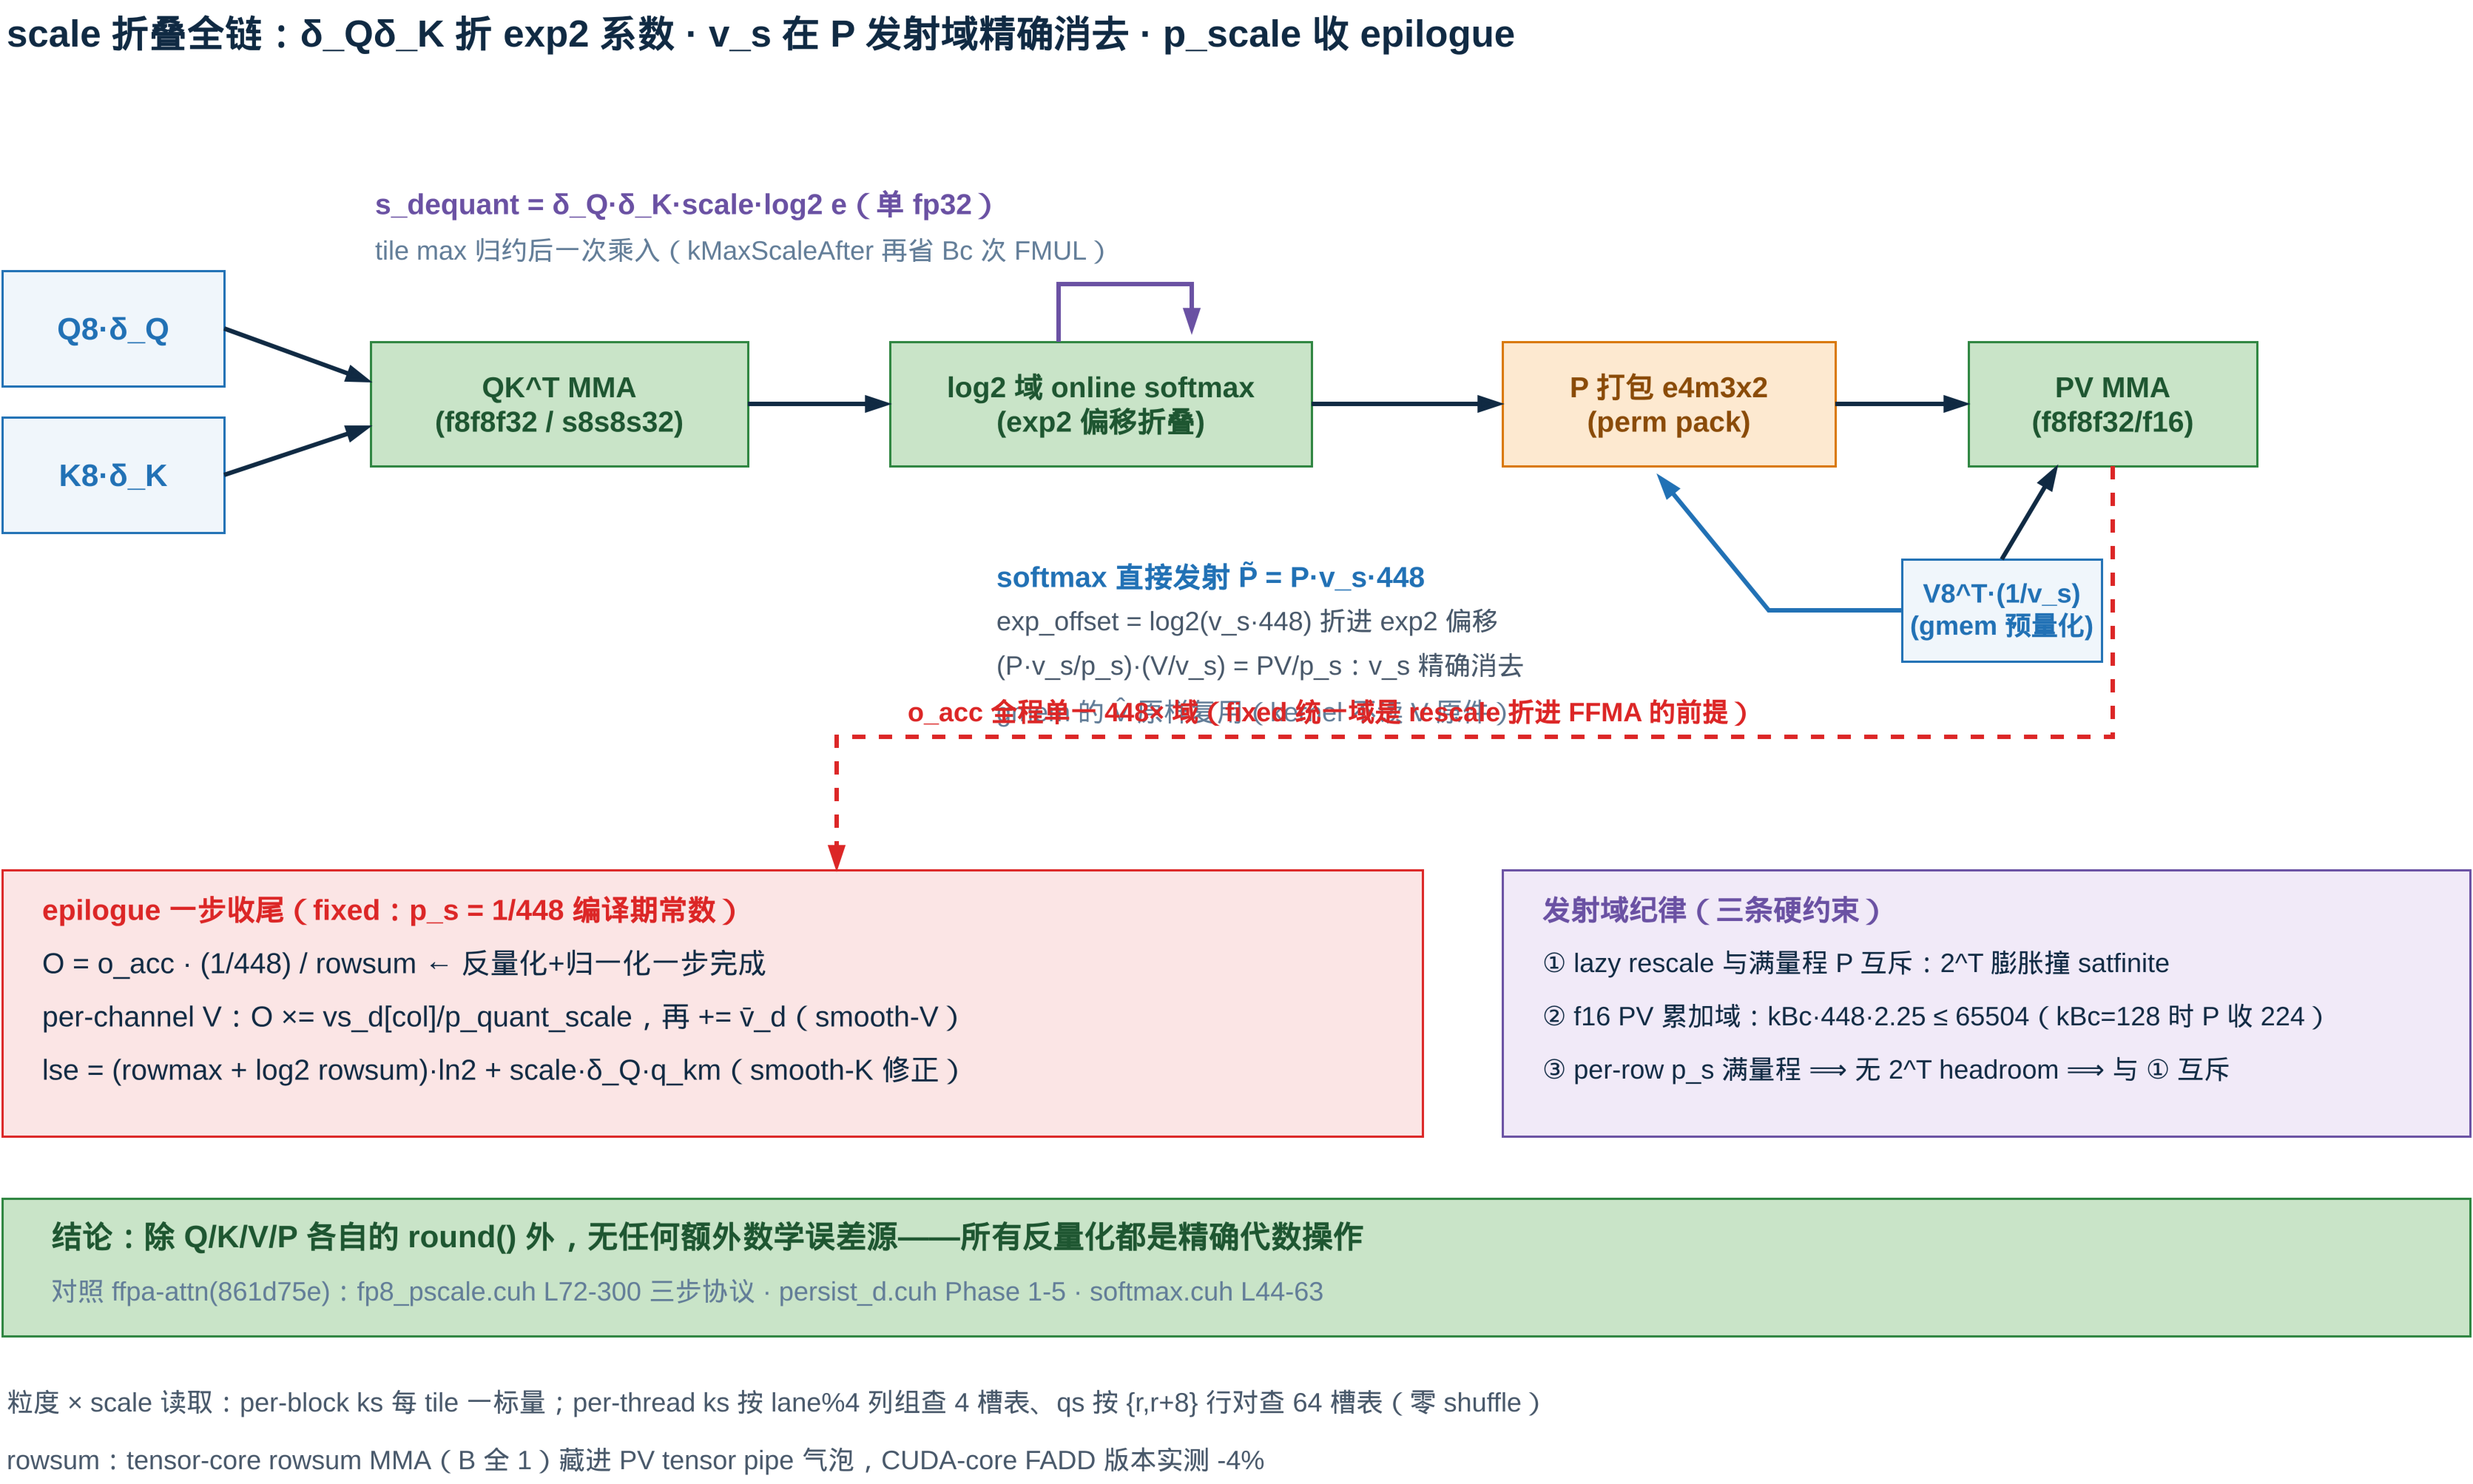
\includegraphics[width=0.98\textwidth]{figures/fig-29-1-scale-folding.png}
  \caption{scale 折叠全链数据流：$\delta_Q\delta_K$ 折进 exp2 系数、$v_s$
  在 P 发射域消去、$p_{scale}$ 收在 epilogue——除 round() 外无额外误差源。}
  \label{fig:29-scale-folding}
\end{figure}

\begin{figure}[H]
  \centering
  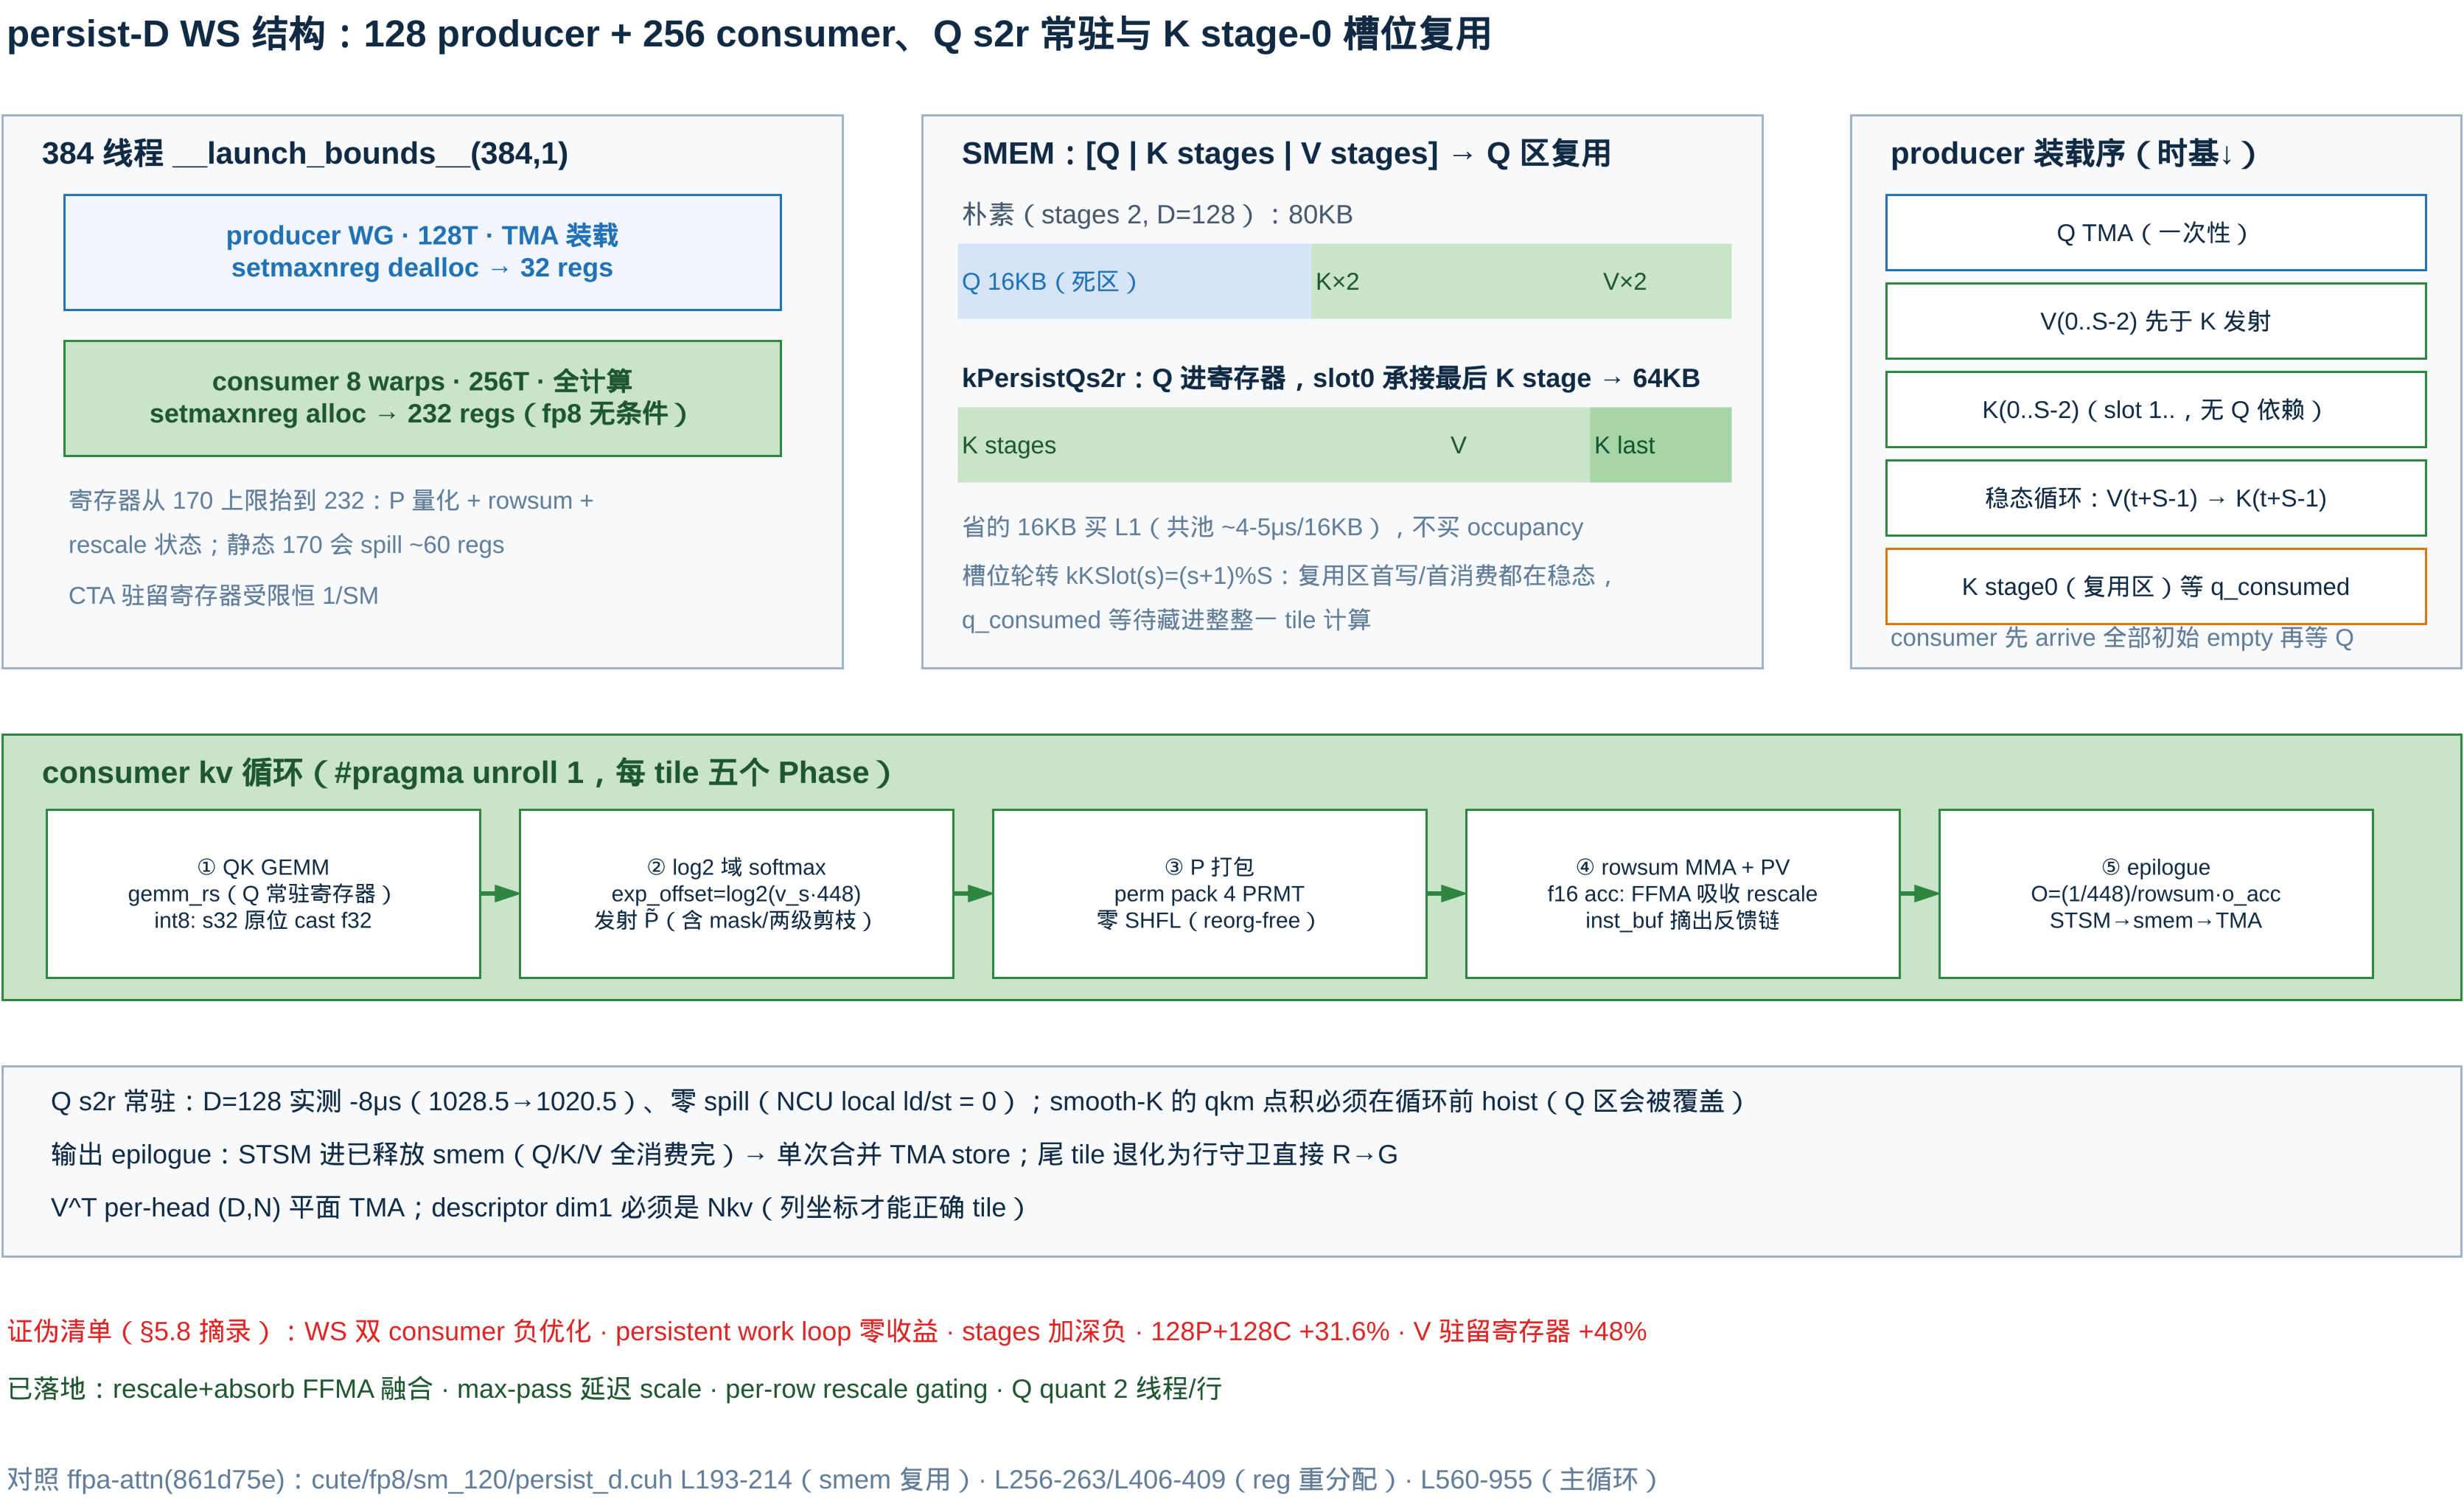
\includegraphics[width=0.98\textwidth]{figures/fig-29-2-persist-d-ws.png}
  \caption{persist-D WS 结构：128P+256C、setmaxnreg 32/232、Q s2r 常驻与
  K stage-0 槽位轮转的 smem 复用、STSM+TMA 输出。}
  \label{fig:29-persist-d-ws}
\end{figure}

\begin{figure}[H]
  \centering
  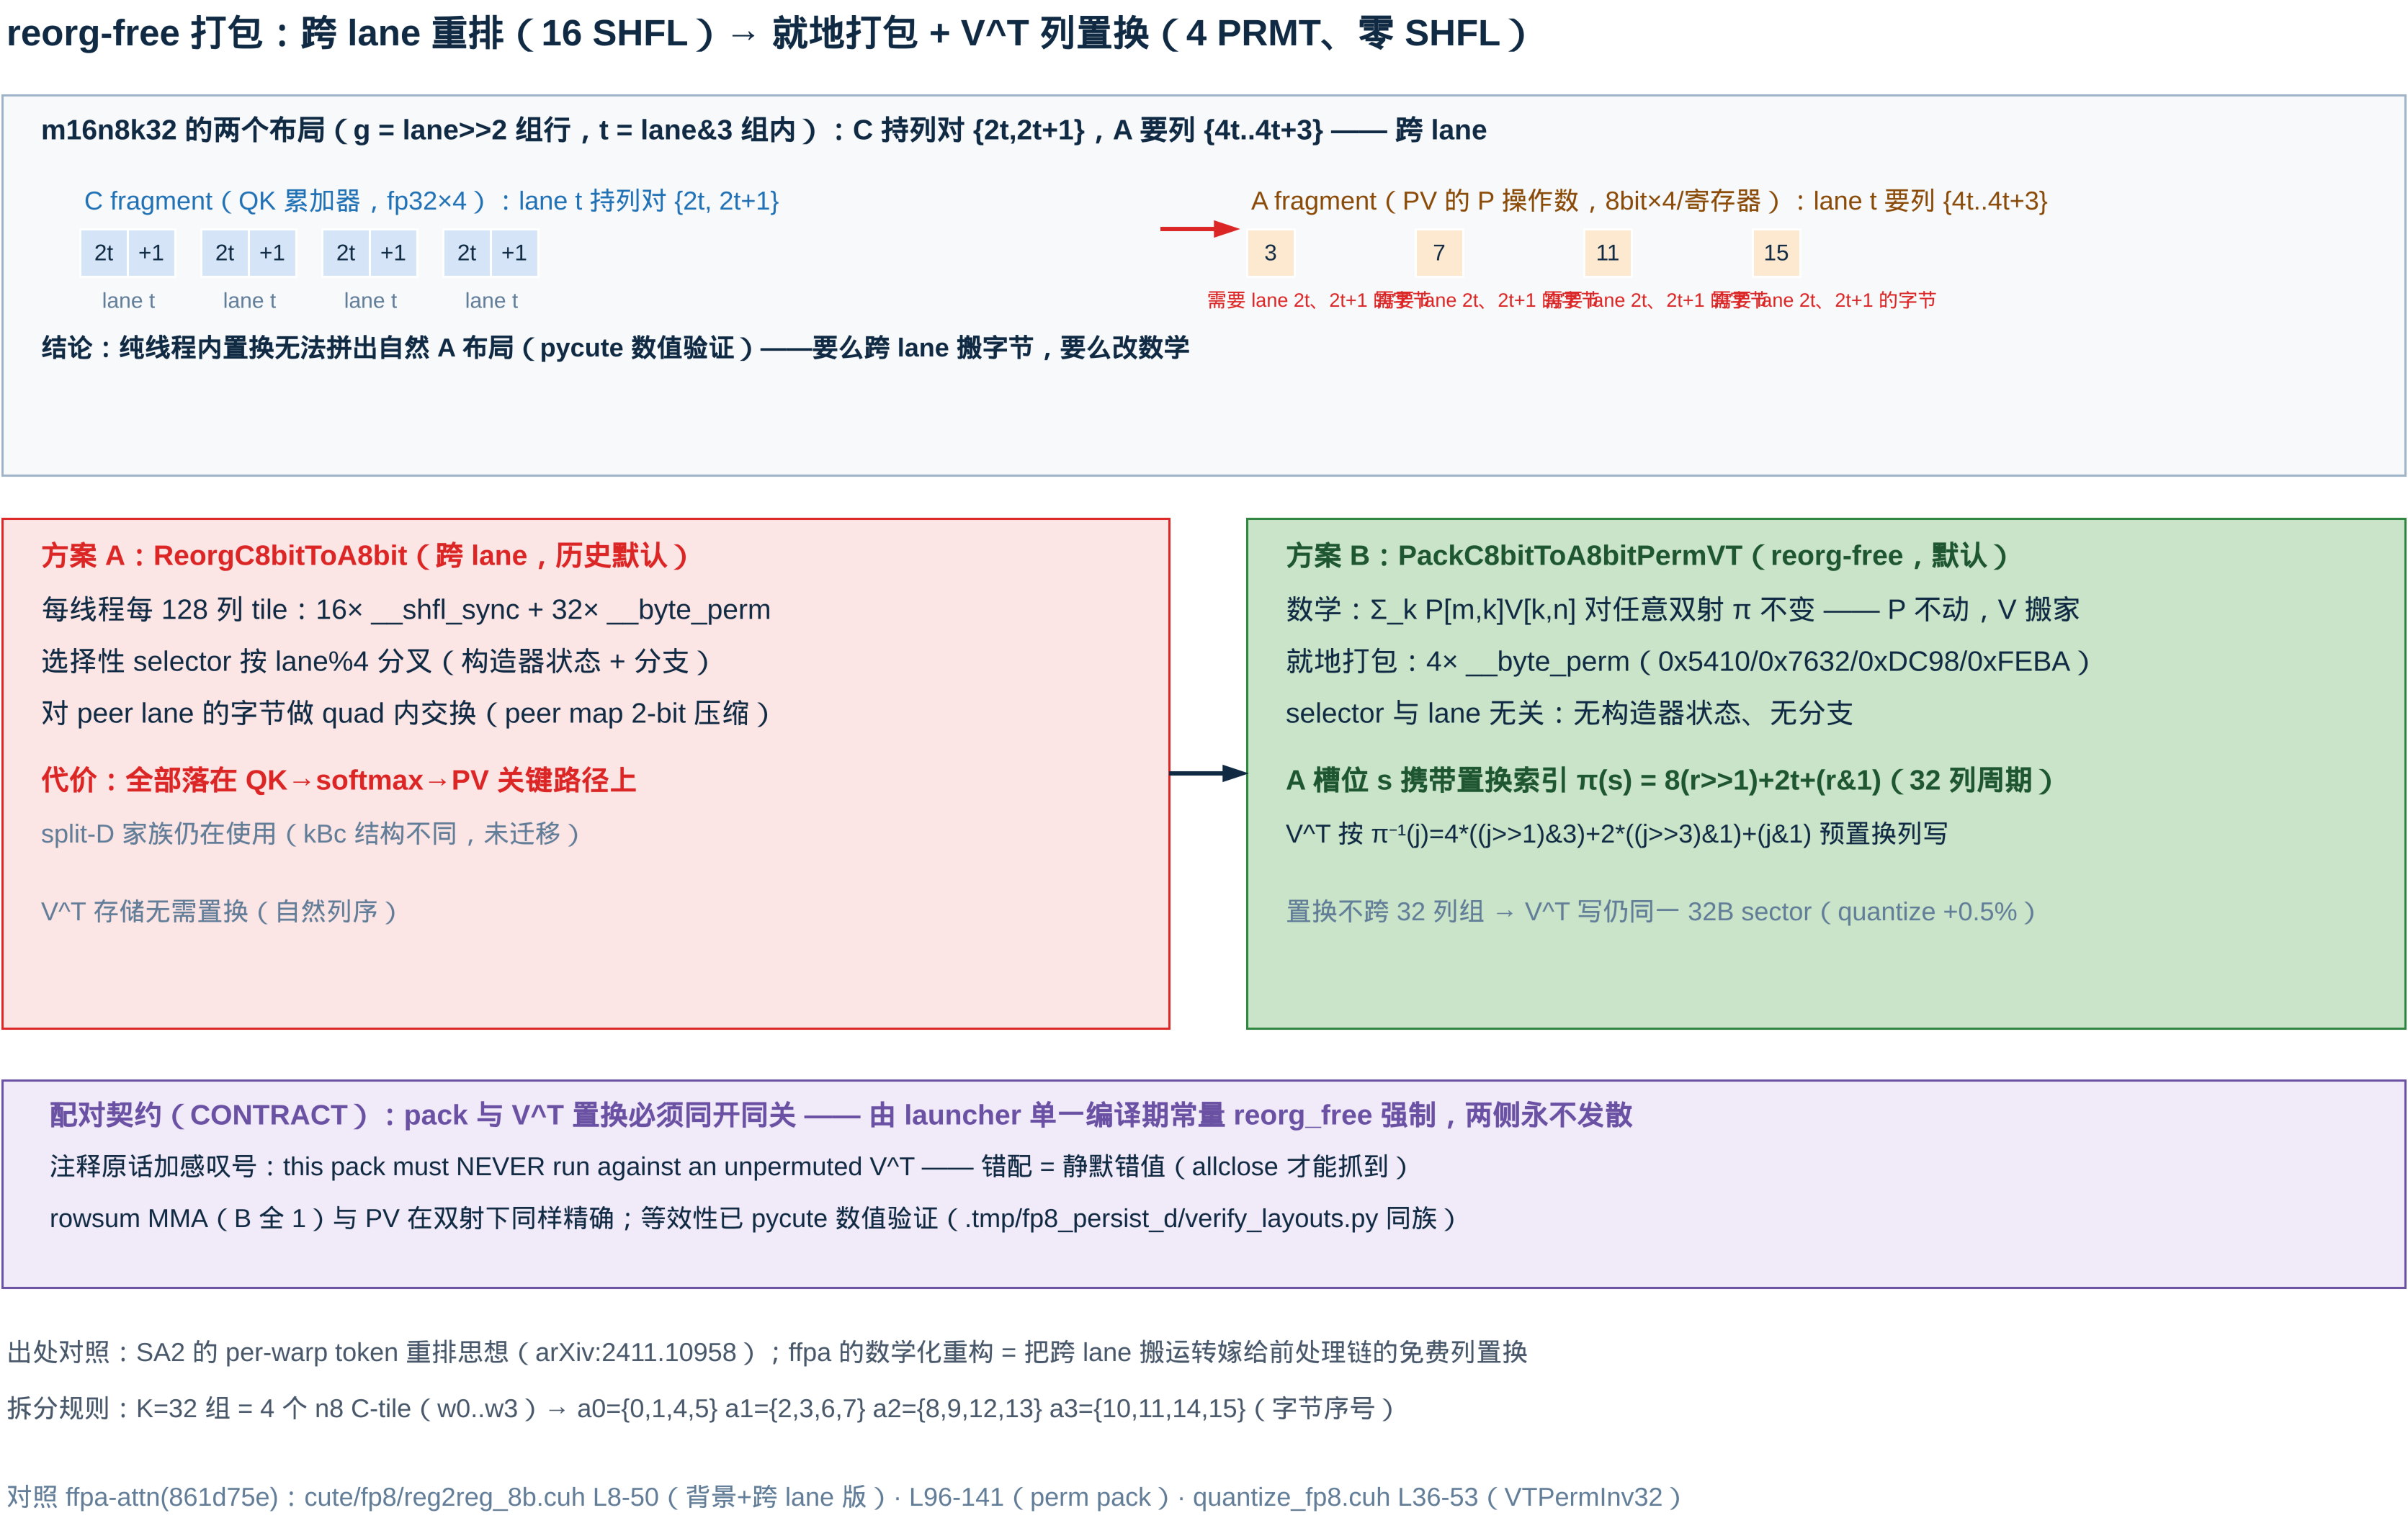
\includegraphics[width=0.98\textwidth]{figures/fig-29-3-reorg-free.png}
  \caption{reorg-free 打包对照：跨 lane 重排（16 SHFL）vs 就地打包 + $V^{\top}$
  列置换（4 PRMT、零 SHFL），归约轴双射不变性保证精确等价。}
  \label{fig:29-reorg-free}
\end{figure}

\section{性能分析}

\subsection{本机实测（RTX PRO 5000，B1 H32 N8192，bench 默认配置）}

\begin{center}
\begin{tabular}{llcccc}
\toprule
$D$ & task & FFPA & SDPA & TFLOPS & speedup \\
\midrule
64  & self-attn & 1.91ms & 2.40ms & 288T & 1.26$\times$ \\
64  & causal    & 1.16ms & 1.34ms & 237T & 1.16$\times$ \\
128 & self-attn & 3.02ms & 5.12ms & 365T & \textbf{1.70$\times$} \\
128 & causal    & 1.85ms & 2.68ms & 297T & 1.45$\times$ \\
192 & self-attn & 4.58ms & 7.27ms & 360T & 1.59$\times$$^{*}$ \\
\bottomrule
\end{tabular}
\end{center}
$^{*}$D=192 存在正确性 bug（29.7.1~节），速度数据仅供参考。D=64 的收益
小于 D=128 是因为 attention 的算术强度随 $D$ 下降、quantize aux 链占比
上升。kernel 级与 SageAttention 对比稳定 $+1.1\sim2.3\%$（仓库 NCU 记录）。

\subsection{微优化到顶：一份「证伪清单」的价值}

persist-D 的结构优化路线已被系统实测证伪（完整清单见仓库 RFC
\S5.8）：WS 双 consumer（FA3 式 2$\times$128T）负优化；persistent work
loop 零收益（tensor-bound 77\%）；stages 加深负（K2V2 预取已领先）；
v2/v3/v5（128P+128C、无 WS、V 驻留寄存器）分别 $+31.6\%$/追平/$+48\%$；
cluster 化无 DSMEM 需求、持平或更慢；CUDA-core row-sum 替代 tensor
rowsum MMA $-4\%$。\textbf{已落地的优化}（D=128）：rescale+absorb FFMA
融合、max-pass 延迟 scale、per-row rescale gating、Q quant 2 线程/行。
这份「负结果清单」与正结果同样重要——它把后续优化方向的搜索空间
压缩到了 engine 层（aux 链 overlap）。

\subsection{带宽与算术的边界}

D=128、N=8192 时主 kernel 365T FLOPS 对应的 DRAM 流量很小（$O(N\cdot D)$
量级 workspace 单遍），瓶颈在 tensor pipe 与 softmax 的依赖链——与
fp16 家族同构，但 fp8 的 MMA 吞吐翻倍使 softmax/P 打包的相对占比上升，
这也是 \texttt{kMaxScaleAfter}、FFMA 吸收融合这类\textbf{指令级}优化
在此路径收益显著的原因。

\section{实践经验}

\subsection{案例：D=192 正确性 bug 的定位（真实故事）}\label{sec:29-d192}

写本章的 bench 验证时发现 \texttt{--cuda-impl fp8 --D 192}
allclose 失败（fp16/bf16 双双 ❌），而 D=64/128 全绿。定位过程本身是
一份方法论示范：
\begin{enumerate}[itemsep=1pt,topsep=2pt]
  \item \textbf{误差量级分类}：max\_abs=2.66 vs mean\_abs=0.011——均值是
        正常 fp8 精度，最大值是灾难级 $\Rightarrow$ \textbf{正确性 bug}
        （个别行错），不是精度不足；
  \item \textbf{行模式定位}：per-row max 直方图显示坏行集中在
        $row\bmod128\in[64,127]$（每个 128 行 Q tile 的后半）；
  \item \textbf{N 缩放}：N=512 时几乎全错、N=8192 时只剩 11\% 行错
        ——错误随 N 稀释，说明错的是\textbf{特定 (row, kv-tile) 组合}而非
        系统性索引错位；
  \item \textbf{配置矩阵消去}：默认/纯 fp8 f32acc/int8+f16acc/no-smK/
        per-thread/per-channel 全部 ❌ $\Rightarrow$ 与量化 knob 无关，
        bug 在 D=192 特有的主 kernel 路径（$kBc{=}64$ 变体、SW64 swizzle、
        或 quantize 侧 kBlockRows 与 kBc 的一致性）；
  \item \textbf{fp16 对照}：fp16 CUTE 路径 D=192 完全正确
        （max=0.0001）$\Rightarrow$ 输入布局/TMA/寻址层无辜，责任圈定在
        fp8 专属代码。
\end{enumerate}
教训：\textbf{「速度好+均值好」不等于正确}——bench 的 allclose 是唯一
硬门槛；误差的 max/mean 分裂是「个别行错」的强信号；行号模 tile 尺寸的
直方图能直接把 bug 锚到 tile 结构的哪一半。

\subsection{考据：sm\_89 的 cp.async 变体}

同文件名在 \texttt{cute/fp8/sm\_89/persist\_d.cuh} 有一个 Ada 变体：
无 TMA/mbarrier，用 sm80 装载协议（cp.async + \texttt{wait<2S-1>}）复用
sm120 的计算层（int8 QK / fixed p\_scale / f8f8f16 PV），256T non-WS。
其 NCU 结论（依赖链/发射受限，\texttt{math\_pipe\_throttle} 1.32 $\gg$
\texttt{wait} 0.82）与深流水零收益的证伪记录，是「同一算法在不同装载
协议下瓶颈漂移」的绝佳对照。本节不展开，读者按需查阅源码头注释。

\section{常见坑}

\begin{enumerate}[itemsep=1pt,topsep=2pt]
  \item \textbf{P 是 online 量化，无法离线校准}：Q/K/V 都能离线 smoothing
        /per-channel 校准，P 每 tile 现算现量化，值域与分布逐行剧变
        （causal 早行近 one-hot、dense 行近均匀）——只能选固定/保守发射域。
        这是量化 attention 精度损失的主要根源之一（实测 P 0.11 与 QK 0.13
        同量级、V 0.19 最大）。
  \item \textbf{满量程 P 与 lazy rescale 互斥}：发射域铺满 448 后 stale max
        的 $2^T$ 膨胀必然 satfinite（29.3.3~节）；fp8 traits 直接关掉
        lazy rescale，且 f16 acc 路径把 rescale 融进吸收 FFMA 后延迟惩罚
        消失。
  \item \textbf{kVTPerm 配对是编译期纪律}：\texttt{PackC8bitToA8bitPermVT}
        对未置换的 $V^{\top}$ 运行 = 静默错值。配对由 launcher 单一常量
        强制；绕过 launcher 直接调 kernel 没有保护。
  \item \textbf{f16 PV 累加域}：$kBc\cdot448\cdot2.25\le65504$ 的编译期
        检查不过时 P 域自动收到 224——不理解这条约束会以为 P 域「有时
        448 有时 224」是随机行为。
  \item \textbf{early rows 的 ESS 幅度放大}（27.3.8~节）：causal 前几行
        ESS$\approx$1、幅度 $3.1\sigma$，fp8 每级 $\sim$5\% 相对误差换算
        成 15$\times$ 于 dense 的绝对误差；「早行 fp16 QK」不解决问题
        （V 量化是最大单项），hybrid 全链 fp16 才有效。
  \item \textbf{D=192（$kBc{=}64$ 变体）当前有正确性 bug}：29.7.1~节的
        定位记录；在修复前避免在生产使用该 headdim 的 fp8 persist-D。
\end{enumerate}

\section{面试要点速查}

\begin{enumerate}[itemsep=1pt,topsep=2pt]
  \item fp8 attention 的所有 scale 是如何消去的？
        （$\delta_Q\delta_K$ 折 exp2 系数；$v_s$ 折 P 发射域精确消去；
        $p_{scale}$ 收 epilogue——式~\ref{eq:29-sdequant}--\ref{eq:29-threestep}。）
  \item 为什么 P 的量化只能 fixed/保守，不能离线校准？
        （P 每 tile 现算、分布逐行剧变；离线对象必须前向开始前存在。）
  \item lazy rescale 与满量程 P 为什么互斥？（$2^T$ 膨胀 vs 448 satfinite，
        29.3.3~节；f16 acc 路径 FFMA 吸收让 rescale 免费。）
  \item f16 PV 累加器的域怎么算？（$\pm65504/32=2047$；P 448 $\times$ V
        2.25 $=1008$ ✓——SA2++ 双侧收窄 vs ffpa 单侧压 V 的差异。）
  \item reorg-free 打包省了什么、代价是什么？（16 SHFL+32 PRMT $\to$
        4 PRMT 零 SHFL；代价 $V^{\top}$ 列置换预写 + 编译期配对纪律，
        式~\ref{eq:29-perm-inv}。）
  \item Q 的 s2r 常驻为什么省钱？省的是 occupancy 吗？
        （不是——省 smem（16KB Q 区复用）$\to$ 买 L1 共池容量，
        $\sim$4--5$\mu s$/16KB；CTA 驻留本就寄存器受限。）
  \item fp8 persist-D 的 D 范围与家族分工？（$\le$224 %32；更大走
        split-D M8N1 / M4N2，第~\ref{ch:30}~章。）
\end{enumerate}

\section{最小测试与动手实验}

\begin{lstlisting}[style=console]
# 环境（Card 7，小 headdim 放行）
$ conda activate cdit
$ export CUDA_VISIBLE_DEVICES=7 FFPA_CUDA_ALLOW_SMALL_D=1

# [A] persist-D 域内全绿组合：D=64 / 128
$ python -m ffpa_attn.bench --fwd-backend cuda --cuda-impl fp8 \
    --tasks self-attn,causal --D 128 --no-bwd --show-allclose
# self-attn fp16  8192/8192  3.02ms  365T  1.70x  allclose ✅
# causal    fp16  8192/8192  1.85ms  297T  1.45x  allclose ✅

# [B] 配置显式声明（int8 QK + f16 PV acc）
$ python -m ffpa_attn.bench --fwd-backend cuda --cuda-impl fp8 \
    --tasks self-attn --D 128 --no-bwd --show-allclose \
    --fp8-qk-mm-type int8 --fp8-pv-acc-type f16
# 3.08ms  357T  1.67x  allclose ✅

# [C] D=192：正确性 bug 复现（29.7.1 节）
$ python -m ffpa_attn.bench --fwd-backend cuda --cuda-impl fp8 \
    --tasks self-attn --D 192 --no-bwd --show-allclose
# allclose ❌  ← 坏行集中在 row%128 ∈ [64,127]
\end{lstlisting}

\textbf{实验 1（scale 流向追踪）}：把 \texttt{persist\_d.cuh} 的
Phase 1--5 各自在纸上标出「哪个 scale 在哪条指令上被乘/消去」，对照
图~\ref{fig:29-scale-folding}——练到能默写三步协议。
\textbf{实验 2（发射域 A/B）}：\texttt{FFPA\_FP8\_PQUANT\_PER\_ROW=1}
重跑 [A]，观察精度提升与速度代价（per-row 归约 + $o\_tile$ 暂存）。
\textbf{实验 3（bug 定位复演）}：按 29.7.1~节步骤用 PyTorch 复现 D=192
的行模式直方图（脚本思路：per-row max diff $>$ 0.1 统计
$row\bmod128$）——把「速度好+均值好 $\neq$ 正确」变成肌肉记忆。
\textbf{实验 4（lazy rescale 证伪）}：读 \texttt{attn\_traits.cuh}
L31--37 注释，回答「为什么 fp8 关掉 lazy rescale 而 fp16 开着」。

\section*{延伸阅读}
\begin{itemize}[itemsep=0pt,topsep=2pt]
  \item SageAttention2（arXiv:2411.10958）：per-warp token 重排与 int8 QK
        的原始出处（reorg-free 打包的对照原型）。
  \item SageAttention2++（arXiv:2505.21136）\S3.1：f16 PV 累加域约束
        （$P_r\times V_r\le2047$）的推导。
  \item FlashAttention-4（arXiv:2603.05451）：lazy rescale 与量化域交互
        （本章 29.3.3~节的反例来源）。
  \item ffpa-attn \texttt{reg2reg\_8b.cuh} 头注释：C$\to$A fragment
        布局的 PTX 级推导与 pycute 数值验证记录。
  \item ffpa-attn 仓库 RFC \S5.8：persist-D 结构优化的完整证伪清单
        （负结果的科学价值）。
\end{itemize}
